\documentclass[a4paper, 11pt]{article}
\usepackage{comment}
\usepackage{lipsum} 
\usepackage{fullpage} %cambiar margen
\usepackage[a4paper, total={7in, 10in}]{geometry}

\usepackage{amssymb,amsthm} 
\usepackage{amsmath}
\newtheorem{theorem}{Theorem}
\newtheorem{corollary}{Corollary}
\usepackage{graphicx}
\usepackage{tikz}
\usetikzlibrary{arrows}
\usepackage{verbatim}
%\usepackage[numbered]{mcode}
\usepackage{float}
\usepackage{tikz}
\usetikzlibrary{shapes,arrows}
\usetikzlibrary{arrows,calc,positioning}
\usepackage{mathpazo} %tipo de letra 
\usepackage[utf8]{inputenc} %codificación
\usepackage[T1]{fontenc} %digitación de tildes y ñ
\usepackage[spanish]{babel} %paquete de soporte español

\tikzset{
	block/.style = {draw, rectangle,
		minimum height=1cm,
		minimum width=1.5cm},
	input/.style = {coordinate,node distance=1cm},
	output/.style = {coordinate,node distance=4cm},
	arrow/.style={draw, -latex,node distance=2cm},
	pinstyle/.style = {pin edge={latex-, black,node distance=2cm}},
	sum/.style = {draw, circle, node distance=1cm},
}
\usepackage{xcolor}
\usepackage{mdframed}
\usepackage[shortlabels]{enumitem}
\usepackage{indentfirst}
\usepackage{hyperref}

\usepackage{listings}
\lstset{literate=
  {á}{{\'a}}1
  {é}{{\'e}}1
  {í}{{\'i}}1
  {ó}{{\'o}}1
  {ú}{{\'u}}1
  {Á}{{\'A}}1
  {É}{{\'E}}1
  {Í}{{\'I}}1
  {Ó}{{\'O}}1
  {Ú}{{\'U}}1
  {ñ}{{\~n}}1
  {ü}{{\"u}}1
  {Ü}{{\"U}}1
}

\lstdefinestyle{customc}{
  belowcaptionskip=1\baselineskip,
  breaklines=true,
  frame=L,
  xleftmargin=\parindent,
  language=Python,
  showstringspaces=false,
  basicstyle=\footnotesize\ttfamily,
  keywordstyle=\bfseries\color{green!40!black},
  commentstyle=\itshape\color{purple!40!black},
  identifierstyle=\color{blue},
  stringstyle=\color{orange},
}

\lstdefinestyle{customasm}{
  belowcaptionskip=1\baselineskip,
  frame=L,
  xleftmargin=\parindent,
  language=[x86masm]Assembler,
  basicstyle=\footnotesize\ttfamily,
  commentstyle=\itshape\color{purple!40!black},
}

\lstset{escapechar=@,style=customc}



\renewcommand{\thesubsection}{\thesection.\alph{subsection}}

\newenvironment{problem}[2][Ejercicio]
{ \begin{mdframed}[backgroundcolor= red!50] \textbf{#1 #2} \\}
	{  \end{mdframed}}

% Define solution environment
\newenvironment{solution}
{\textcolor{blue}{\textbf{\textit{Solución:\\\noindent}}}}


\renewcommand{\qed}{\quad\qedsymbol}

% \\	
\begin{document}
	\noindent
	%%%%%%%%%%%%%%%%%%%%%%%%%%%%%%%%%%%%
	
	\begin{minipage}[b][1.2cm][t]{0.8\textwidth}
		\large\textbf{César Isaí García Cornejo} \hfill \textbf{Tarea 2}  \\
		cesar.cornejo@cimat.mx \hfill \\
		\normalsize Estadística Bayesiana \hfill Semestre 4\\
	\end{minipage}
	
	\hspace{14.4cm}
	\begin{minipage}[b][0.03cm][t]{0.12\linewidth}
		
		\vspace{-2.2cm}
		%%%La Ruta dependerá de donde este alojado el main y la imagen
		
\includegraphics[scale=0.3]{Figures/EscudoCimat.png}
	\end{minipage}
	
	\noindent\rule{7in}{2.8pt}
	
	%%%%%%%%%%%%%%%%%%%%%
	%%%%%%%%%%%%%%%%%%%%%%%%%%%%%%%%%%%%%%%%%%%%%%%%%%%%%%%%%%%%%%%%%%%%%%%%%%%%%%%%%%%%%%%%%%%%%%%%%%%%%%%%%%%%%%%%%%%
	% Problem 1
	%%%%%%%%%%%%%%%%%%%%%%%%%%%%%%%%%%%%%%%%%%%%%%%%%%%%%%%%%%%%%%%%%%%%%%%%%%%%%%%%%%%%%%%%%%%%%%%%%%%%%%%%%%%%%%%%%%%%%%%%%%%%%%%%%%%%%%%%
	\setlength{\parskip}{\medskipamount}
	\setlength{\parindent}{0pt}
%/////////// Ejercicio 1 /////////////////
\begin{problem}{1} 
    Suponga que $X_i \sim U(0,\theta)$ independientes. ¿Cómo haría inferencia bayesiana (conjugada) sobre $\theta$ para analizar la Hipótesis $H_0: \theta < 20$ vs $H_1: \theta \geq 20$? Ejemplo: Tenemos un equipo electrónico cuya confiabilidad se puede describir con una distribución uniforme. Los tiempos de falla en meses de 30 de estos aparatos son: 7.7, 1.2, 5.5, 5.5, 13.0, 12.0, 9.7, 11.0, 18.0, 19.0, 16.0, 9.3, 6.8, 3.7, 4.8, 6.1, 2.2, 3.6, 9.9, 8.0, 19.0, 11.0, 15.0, 8.1, 15.0, 5.1, 12.0, 7.3, 2.1, 14.0. ¿Qué se puede concluir entonces del contraste de hipótesis anterior?    
\end{problem}

\begin{solution} 
    Dado que se nos pide hacer una análisis conjugado para un modelo donde $X_i \sim U(0,\theta)$ entonces es que se tiene que proponer una distribución a priori $\theta \sim Pareto(\alpha_0,\beta_0)$. Mostraremos que en efecto estamos ante un análisis conjugado. Primeramente, recordemos que la densidad de una distribución $Pareto(\alpha,\beta)$ es
    \begin{align}
        f(x) = \alpha \beta ^\alpha x^{-(\alpha +1)} \mathbb{1}_{[\beta,\infty)}(x).
        \label{Pareto}
    \end{align}
    Notemos que el soporte de la distribución Pareto depende del parámetro $\beta$.

    Por otro lado, la distribución posterior del parámetro $\theta$ es
    \begin{align}
        f(\theta|X^n) \propto f(\theta) \mathcal{L}(\theta)
    \end{align}
    con la distribución a priori $\theta \sim Pareto(\alpha_0,\beta_0)$ se sigue que
    \begin{align*}
        f(\theta|X^n) \propto \alpha_0 \beta_0^{\alpha_0} \theta^{-(\alpha_0 +1)} \mathbb{1}_{[\beta_0,\infty)}(\theta) \prod_{i = 1}^{n} \frac{1}{\theta} \mathbb{1}_{[0,\theta]}(X_i).
    \end{align*}
    Observemos que la verosimilitud se anula si existe un $i$ tal que $X_i > \theta$. Entonces, para tener verosimilitud no nula se requiere que para todo $i$ se cumpla $\theta \geq X_i$. Dicho de otra forma, basta con que se cumpla que $\theta \geq X_{(n)}$ donde $X_{(n)} = max_{i}\{X_i\}$ también conocida como la estadística de orden superior. Por tanto,
    \begin{align*}
        f(\theta|X^n) \propto \theta^{-(\alpha_0 + n +1)} \mathbb{1}_{[\beta_0,\infty)}(\theta) \mathbb{1}_{[X_{(n)}, \infty)}(\theta)
    \end{align*}
    Recordemos que el producto de dos funciones indicadores sobre dos conjuntos es la función indicadora de la intersección. Así
    \begin{align}
        f(\theta|X^n) \propto \theta^{-(\alpha_0 + n +1 )} \mathbb{1}_{[\max\{X_{(n)}, \beta_0\}, \infty)} (\theta)
        \label{1.03}
    \end{align}
    Contrastando (\ref{1.03}) con (\ref{Pareto}) que es el kernel de una distribución Pareto, lo que muestra que en efecto son familias conjugadas. 
    
    Por tanto, la distribución posterior es también una distribución Pareto
    \begin{align}
        \theta|X^n \sim Pareto(\alpha_p, \beta_p)
    \end{align}
    donde $\alpha_p = \alpha_0 + n$ y $\beta_p = \max \{\beta_0, X_{(n)}\}$ 

    Previo a ver los datos, no tenemos conocimiento sobre $\theta$. Como se propondrá un distribución a priori Pareto, y el parámetro $\beta$ controla el soporte de forma que $\theta \in [\beta,\infty)$. Conviene proponer una distribución cuyo soporte sean los reales no negativos, esto pasaría con la distribución Pareto solo si $\beta$ es cercano a cero. Por tanto elegimos $\beta = 1$. Para el parámetro $\alpha$, tenemos distribuciones más \textit{delgadas} para mayores valores de $\alpha$. Luego, elegimos un valor pequeño, sin embargo, para $\alpha \leq 1$ no tiene media y para $\alpha \leq 2$ no tiene varianza. Por ello seleccionamos para la distribución a prior $\alpha = 5$.

    Así, la distribución a priori es 
    \begin{align*}
        \theta \sim Pareto(\alpha_0 = 5, \beta_0 = 1)
    \end{align*}
    Como $\alpha_p = \alpha_0 + n = 35$ y $\beta_p = \max\{\beta_0,X_{(n)}\}=\max\{1,19\} = 19$, la distribución posterior es
    \begin{align}
        \theta|X^n \sim Pareto(\alpha_p = 35, \beta_p = 19)
    \end{align}
    Notemos que el soporte de la distribución posterior decreció y ademas se tiene una distribución más \textit{concentrada}.

    \begin{figure}[H] 
        \centering 
        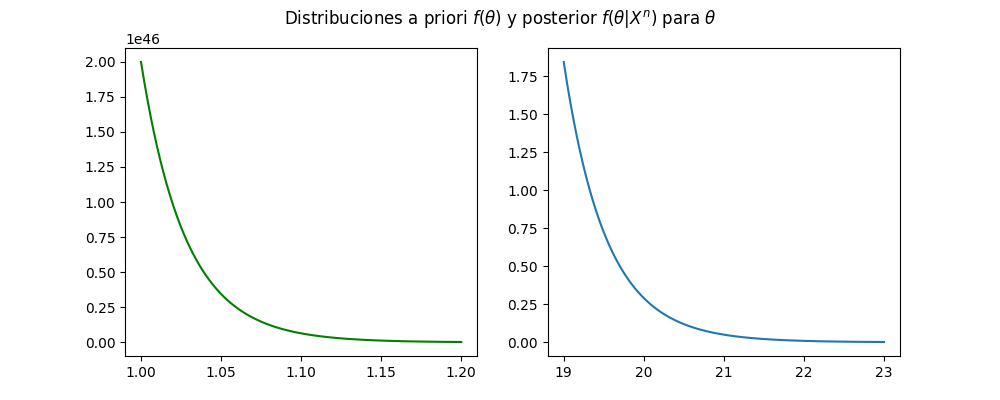
\includegraphics[width = 15 cm]{Figures/distribuciones.png} 
        \caption{Distribución a priori y distribución posterior para $\theta$.}
        \label{Fig. 1.1}
    \end{figure} 
    
\end{solution}


\begin{problem}{2} 
    Si $\mathbf{Y} \sim N_n(\mathbf{X}\theta, \Sigma)$ y $\Sigma$, la matriz de varianzas y covarianzas, conocida (definida positiva); $\mathbf{X}$, la matriz de diseño en la regresión, conocida. Encuentre la posterior $\theta$ usando una $N_p(\mu_0,\Sigma_0 )$ como \textit{a priori}. Encuentre la distribución predictiva de un dato futuro $Y_{n+1}$.
\end{problem}

\begin{solution} 
    
\end{solution}

\newpage

\begin{problem}{3} 
    Sea el modelo de crecimiento logístico $\frac{dX}{dt} = \theta_1 X \left( \theta_2 - X  \right)$ con $X(0) = X_0$. Suponga que tenemos observaciones $y_i$ para $X(t_i), t_1 < t_2 < \cdots < t_n$, con ruido gaussiano aditivo independiente, esto es
    \begin{align*}
        y_i = X(t_i) + \epsilon_i; \:\:\:\:\: \epsilon_i \sim N(0,\sigma), \:\:\: i = 1,2,\cdots,n.
    \end{align*} 
    Simule datos con $X(0) = 100$, $\theta_1 =$ 0.001, $\theta_2 = $ 1000, $\sigma = 30$ , $n= 26$ equiespaciados en $t \in [0,10]$. Haga inferencia bayesiana para los parámetro $\theta_1, \theta_2$. Utilice a priories Gamma, centradas en los valores verdaderos. ¿Qué puede decir de la tasa de crecimiento que es $\lambda = \theta_1\theta_2$ ?
\end{problem}















% \begin{thebibliography}{9}

%     \bibitem{Casella}
%     Robert, C. P., Casella, G., and Casella, G. (1999). Monte Carlo statistical methods (Vol. 2). New York: Springer.

%     \bibitem{Wasserman}
%     Wasserman, L. (2004). All of statistics: a concise course in statistical inference (p. 413). New York: Springer.
    
% \end{thebibliography}
      

\end{document}